\section{Algorithm implementation}
Next, we will implement the three chosen algorithms: MLP (Multilayer Perceptron), Autoencoder, and [Third Algorithm]. These algorithms have been selected due to their suitability for classification problems and their ability to handle structured and complex datasets. First, we will provide a brief introduction to each algorithm, highlighting their key characteristics. After that, we will proceed with the implementation and performance analysis for our dataset.

\subsection{Multilayer Perceptron (MLP)}

The \textbf{Multilayer Perceptron (MLP)} is a core model in the field of machine learning, used for both classification and regression tasks. MLP consists of three primary layers: the \textbf{input layer}, one or more \textbf{hidden layers}, and the \textbf{output layer}. Each layer contains multiple neurons, and neurons from one layer are fully connected to neurons in the next layer. This dense connectivity allows MLP to capture complex relationships in data, particularly non-linear ones, which are common in many real-world applications \cite{deeplearning1}.

In the context of our dataset, which includes health-related features such as \texttt{BMI}, \texttt{Age}, \texttt{Physical\_Health}, and \texttt{Sleep\_Time}, MLP is well-suited to identify hidden patterns and make predictions about whether an individual has diabetes or not. The network learns from the data through a process called \textit{backpropagation}, where errors from the output are propagated back through the network to adjust the weights of the connections between neurons. This process is combined with \textit{gradient descent}, an optimization technique that minimizes the prediction error by adjusting the weights during each iteration of training. Over time, the model learns the optimal weights, improving its ability to make accurate predictions \cite{nn1}.

The basic structure of an MLP is illustrated in the figure below. The input features, such as \texttt{BMI} and \texttt{Age}, are fed into the input layer. From there, they pass through one or more hidden layers, where neurons transform the data by applying learned weights and activation functions. The transformed data then flows to the output layer, which produces the final prediction, such as whether an individual has diabetes.

\begin{figure}[H]
    \centering
    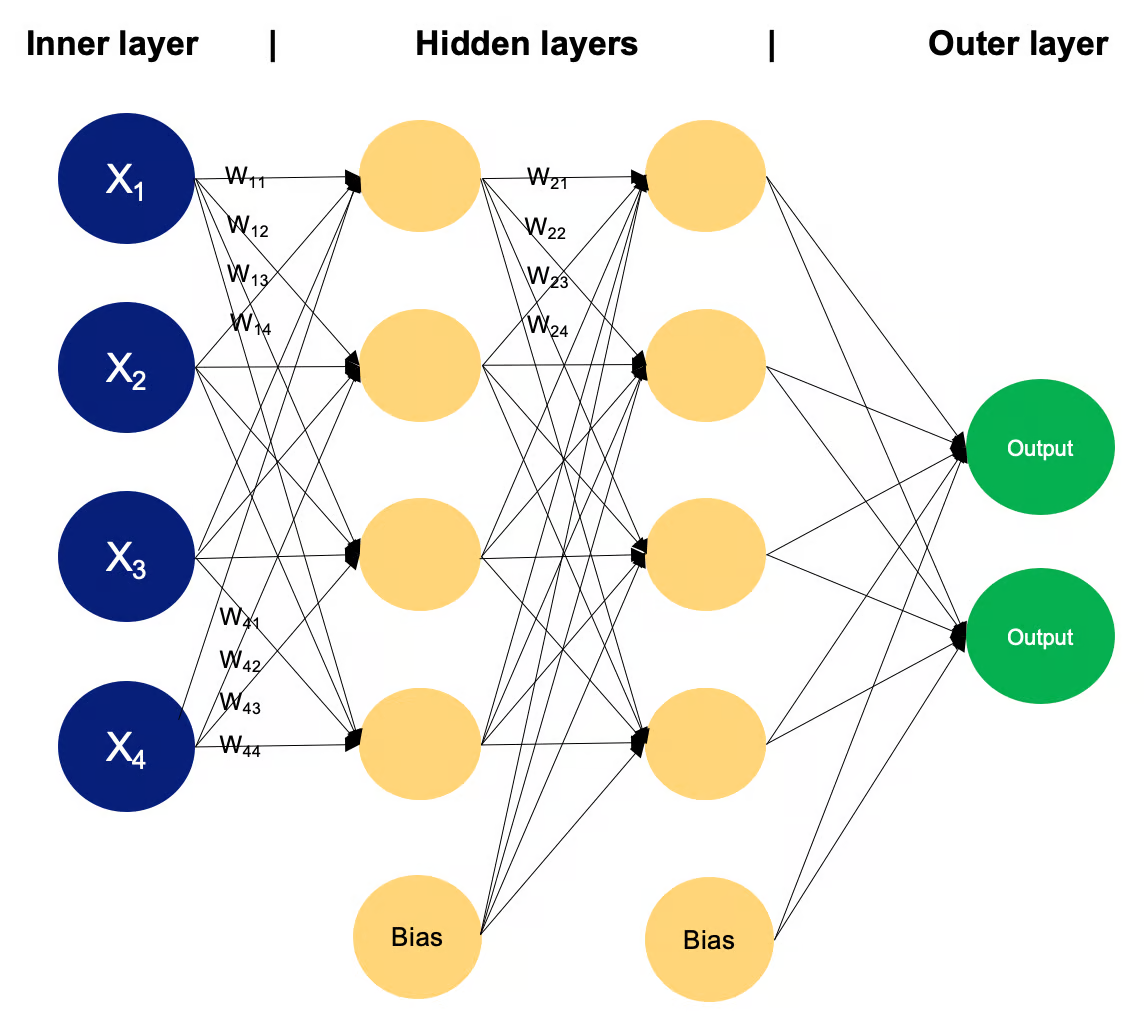
\includegraphics[width=0.7\textwidth]{images/mlp-diagram.png}
    \caption{Basic structure of a Multilayer Perceptron (MLP) \cite{mlp}.}
    \label{fig:mlp}
\end{figure}

In the image, you can observe the flow of information from the input layer through the hidden layers to the output layer. Each layer plays a critical role in transforming the input data to make sense of the patterns and relationships. The neurons in the hidden layers learn features in the data, and as the network adjusts its weights through training, it becomes more accurate in predicting the target outcome.

MLPs are particularly effective in tasks where the relationships between input features and the target variable are non-linear, as is the case in health-related predictions like diabetes classification \cite{deeplearning1}. This model's ability to learn from complex and large datasets allows it to handle a wide variety of problems, from image recognition to medical diagnoses.

What makes MLPs particularly well-suited for our dataset is their capacity to model intricate relationships between multiple features simultaneously. By learning these relationships, MLPs can make accurate predictions, even when the data contains complex, interdependent factors. This makes MLP an ideal choice for predicting the likelihood of diabetes based on a variety of health indicators \cite{mlp}.


\subsection{Autoencoder}

\subsection{Third algorithm}